\documentclass[12pt,a4paper]{article}
\usepackage[utf8]{inputenc}
\usepackage[english,russian]{babel}
\usepackage{indentfirst}
\usepackage{misccorr}
\usepackage{graphicx}
\usepackage{amssymb}
\usepackage{amsmath}

\begin{document}

\begin{center}
    \large
    Работа 1.2.3
    
    Сибгатуллин Булат, Б01-007
    
    \vspace{0.5cm}
    \textbf{Определение моментов инерции твердых тел с помощью трифилярного подвеса}

\end{center}

\vspace{0.5cm}
\textbf{Цель работы:} измерение момента инерции ряда тел и сравнение результатов с расчетами по теоретическим формулам. Проверка адаптивности моментов инерции и справедливости формулы Гюйгенса-Штейнера.

\vspace{0.5cm}
\textbf{В работе используются:} Трифилярный подвес, секундомер, счетчик числа колебаний, набор тел.

Для однородных тел известной плотности при заданных размерах и достаточно простой форме момент инерции можно вычислить при помощи формулы:

\[I = \int r^2 dm\]

Для тел сложной формы при вычислении их момента инерции используют Трифилярный подвес (Рис. 1). Груз кладется на платформу \textit{P'}, её можно привести в движение путем небольшого поворота платформы \textit{P} на угол $\varphi$. В результате этого действия платформа начнет совершать крутильные колебания.

Зная угол $\varphi$ и массу платформы с телом $m$ можем записать закон сохранения энергии при колебаниях:

\begin{equation}\label{1}
\frac{I \dot{\varphi}^2}{2} + mg(z_0 - z) = E
\end{equation}

Здесь $z_0$ - координата по вертикали центра нижней платформы \textsc{O'} при равновесии $\varphi_0 = 0$, а $z$ -  координата той же точки, при угле поворота $\varphi$.

Воспользуемся системой координат \textit{x, y, z,} связанной с верхней платформой (\textit{P}). Координаты точки \textit{С} - (\textit{r},0,0), \textit{C'} - (\textit{R},0,$z_0$). При повороте точка \textit{C'} переходит в точку с координатами \textit{C''} с координатами ($R\cos \varphi$, $R\sin\varphi$,$z$). Расстояние между точками равно длине нити \textit{L}, поэтому можем записать:

\begin{equation}\label{2}
(R\cos\varphi - r)^2 + (R\sin\varphi)^2+z^2 = L^2
\end{equation}

\begin{figure}[h!]
\centering
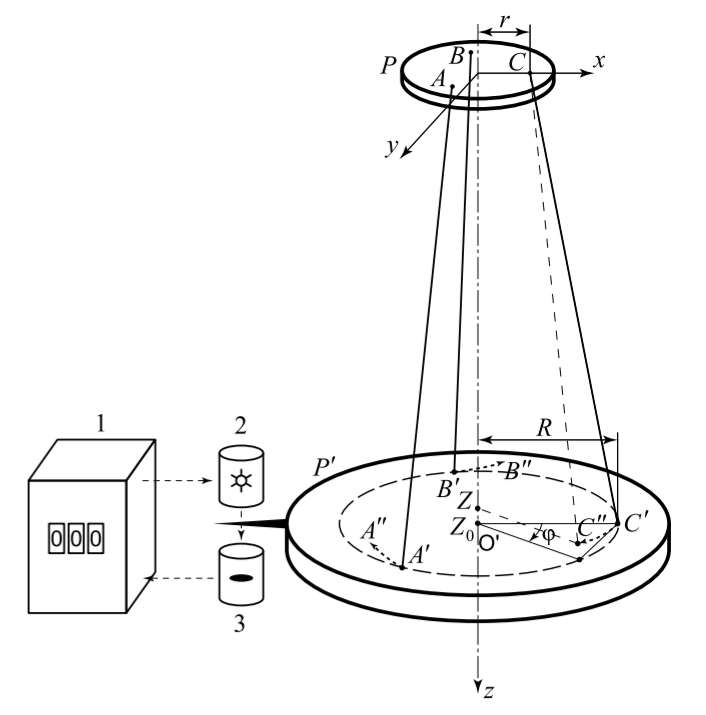
\includegraphics[scale=0.7]{Trifilar suspension.png}
\caption{Трифилярный подвес}
\label{fig:Trifilar suspension}
\end{figure}

\vspace{0.5cm}

Учитывая, что при малых углах поворрота $\cos\varphi \approx 1-\varphi^2 /2$, получим:

\begin{equation}\label{3}
z^2 = L^2-R^2-r^2+2Rr\cos\varphi = z_0^2 - 2Rr(1-\cos\varphi) \approx z_0^2 -Rr\varphi^2
\end{equation}

Преобразуя уравнение (\ref{3}) и подставляя его в уравнение (\ref{1}), получим:

\begin{equation}\label{4}
\frac{1}{2}I\dot{\varphi}^2 + mg\frac{Rr}{2z_0}\varphi^2 = E
\end{equation}

Дифференцируя по времения и сокращая на $\dot{\varphi}$, находим уравнение крутильных колебаний. Производная по времени $E$ равна нулю, поэтому можем сразу найти решение этого уранения:

\begin{equation}\label{5}
\varphi=\varphi_0\sin \Big(\sqrt{\frac{mgRr}{Iz_0}}t + \theta\Big)
\end{equation}

Амплитуда $\varphi_0$ и фаза $\theta$ определяются начальными условиями. Зная период крутильных колебаний системы:

\begin{equation}\label{6}
T = 2\pi \sqrt{\frac{Iz_0}{mgRr}}
\end{equation}

Находим формулу для определения момента инерции:

\begin{equation}\label{7}
I = \frac{mgRrT^2}{4\pi^2z_0}
\end{equation}

Так как параметры установки $z_0, R$ и $r$ при проведении опытов не меняются, удобно переписать последнее уравнение следующим образом:

\begin{equation}\label{8}
I = kmT^2
\end{equation} 

Здесь \textit{k} - величина, постоянная для данной установки равна:

\[k = \frac{gRr}{4\pi^2 z_0}\]

Таким образом, используя данную формулу, мы можем посчитать момент инерции тела с платформой, и платформы отедельно. Затем, пользуясь аддитивностью, вычислить момент инерции тела.

\vspace{0.5cm}

Измерим параметры установки: $z_0 = 215\pm 2$ см, $R = 114,6 \pm 0,5$ см, $r = 30,2 \pm 0,3$ мм.

Константа установки равна:

\[k = \frac{9,81 \cdot 1,146 \cdot 0,0302}{4 \cdot 9,8596 \cdot 2,15}= 4 \cdot 10^{-3} \: \frac{\textit{м}^2}{\textit{с}^2}\]

Определим погрешность измерения k:

\[\sigma_k = k \cdot \sqrt{\Big(\frac{\sigma_R}{R}\Big)^2 + \Big(\frac{\sigma_r}{r}\Big)^2 + \Big(\frac{\sigma_{z_0}}{z_0}\Big)^2} = 5,72 \cdot
 10^{-5} \: \frac{\textit{м}^2}{\textit{с}^2}\]
 
Найдем момент инерции ненагруженной платформы:

\[I_0 = k m_0 T_0^2\],

где $m_0$ - масса платформы, равная $m_0 = 448 \pm 0,3$ \textit{г}, а $T_0$ период колебаний ненагруженной платформы.

Найдем момент инерции платформы со стержнем:

\[I_1 = k (m_0 + m) T_1^2\],

где $m$ - масса стержня, равная $m = 1184,3$ \textit{г}, а $T_1$ - период колебаний системы состоящей из платформы и стержня. Длину стержня $l = 172$, а его поперечный радиус $r = 30$.

Выпишем формулы для нахождения момента инерции стержня. Момент инерции стержня без учета толщины:

\[I_l = \frac{1}{12}ml^2\]

Здесь \textit{l} - длина стержня.

Момент инерции стержня с учетом толщины:

\[I_{kr} = \frac{1}{12}ml^2 + \frac{1}{4}mr^2\]

Здесь \textit{l} - длина стержня, \textit{r} - его радиус.

Так как при подсчете момента инерции экспериментальным путем, мы получим значение момента инерции с учетом толщины, то определим, с какой точностью требуется измерять период колебаний, чтобы обнаружить различие между полученным значением, значением, которой будет подсчитано при помощи табличной формулы для стержня без учета толщины.

Тогда значение момента инерции полученной при помощи опыта будет равно:

\[I_{kr} = I_1 - I_0 = k(m_0 + m) T_1^2 - k m_0 T_0^2\]

Относительные погрешности измерения $T_0$ и $T_1$ возьмем равными друг другу, для удобства подсчета.

Тогда погрешность измерения $I_{kr}$ будет равна:

\[\sigma_{I_{\textit{итог}}} = I_{kr} \cdot \sqrt{\Big(\frac{\sigma_{T_0}}{T_0}\Big)^2 + \Big(\frac{\sigma_{T_1}}{T_1}\Big)^2 + \Big(\frac{\sigma_k}{k}\Big)^2 + \Big(\frac{\sigma_{m_0}}{m_0}\Big)^2} = I_{\textit{итог}} \cdot \sqrt{2 \cdot \varepsilon_T^2 + \Big(\frac{\sigma_k}{k}\Big)^2 + \Big(\frac{\sigma_{m_0}}{m_0}\Big)^2}\]

И $\sigma_{I_{kr}}$ должно быть меньше, чем $I_{l,r} - I_l$:

\[\sigma_{I_{kr}} < \frac{1}{4}mr^2\]

Из этого соотношения можем найти искомое значение $\varepsilon_T$:

\[\varepsilon_T < \sqrt{\frac{1}{2}\Big(\frac{mr^2}{4I_{kr}^2} - \Big(\frac{\sigma_k}{k}\Big)^2 - \Big(\frac{\sigma_{m_0}}{m_0}\Big)^2\Big)}\]

Зная все требуемый значения, можем численно определить $\varepsilon_T$:

\[\varepsilon = 0,2\%\]

Оценочный период колебаний пластины со стержнем будет равен:

\[T_1 = \sqrt{\frac{I_{kr} + I_0}{k(m_0 + m)}} = 0.966 \: \textit{с}\]

Зная, что цена деления равна 0,01 \textit{с}, а дополнительная погрешность измерения времени равна примерно 0,2 \textit{с}, можем найти, что:

\[\frac{0,21}{0,966 \cdot x} = 2 \cdot 10^{-3}\]

Здесь \textit{x} - количество колебаний, и $x = 109$.

\end{document}